\section{\ce{[Zn(dca)_2(4-methoxypyridine)_2]_n}}
\subsection{Synthesis}
20 mL distilled \ce{H_2O} were used as a solvent for 0.30 g \ce{Zn(NO_3)_2 * 6 H_2O} (1 mmol), 0.18 g Na-dicyanamide (2 mmol) and 0.22 g 4-methoxypyridine (2 mmol). The solution was heated up to $80^\circ$C  and stirred for 1 hour. After filtration, the clear  solution was put in the drying oven at $80^\circ$C overnight and then slowly cooled down to 20$^\circ$ in a waterbath. A few hours later white crystals were obtained.
Anal. Calculated for \ce{C_{16}H_{14}N_8O_2Zn} (415.74 g/mol) : 46.28\% C; 3.40\% H; 26.98\% N;
Found: 46.23 \% C; 3.43\% H; 26.98 \% N;
 IR (ATR, cm$^{-1}$): 2294 (m), 2233 (m), 2170 (s), 1922 (w), 1667 (w), 1611 (s), 1566 (s), 1512 (s), 1433 (s), 1345 (s), 1304 (vs), 1206 (s), 1056 (m), 1008 (s), 936 (m), 830 (s), 814 (s), 673 (m), 571 (w), 526 (s), 463 (m)

\begin{figure}[h!]
\centering
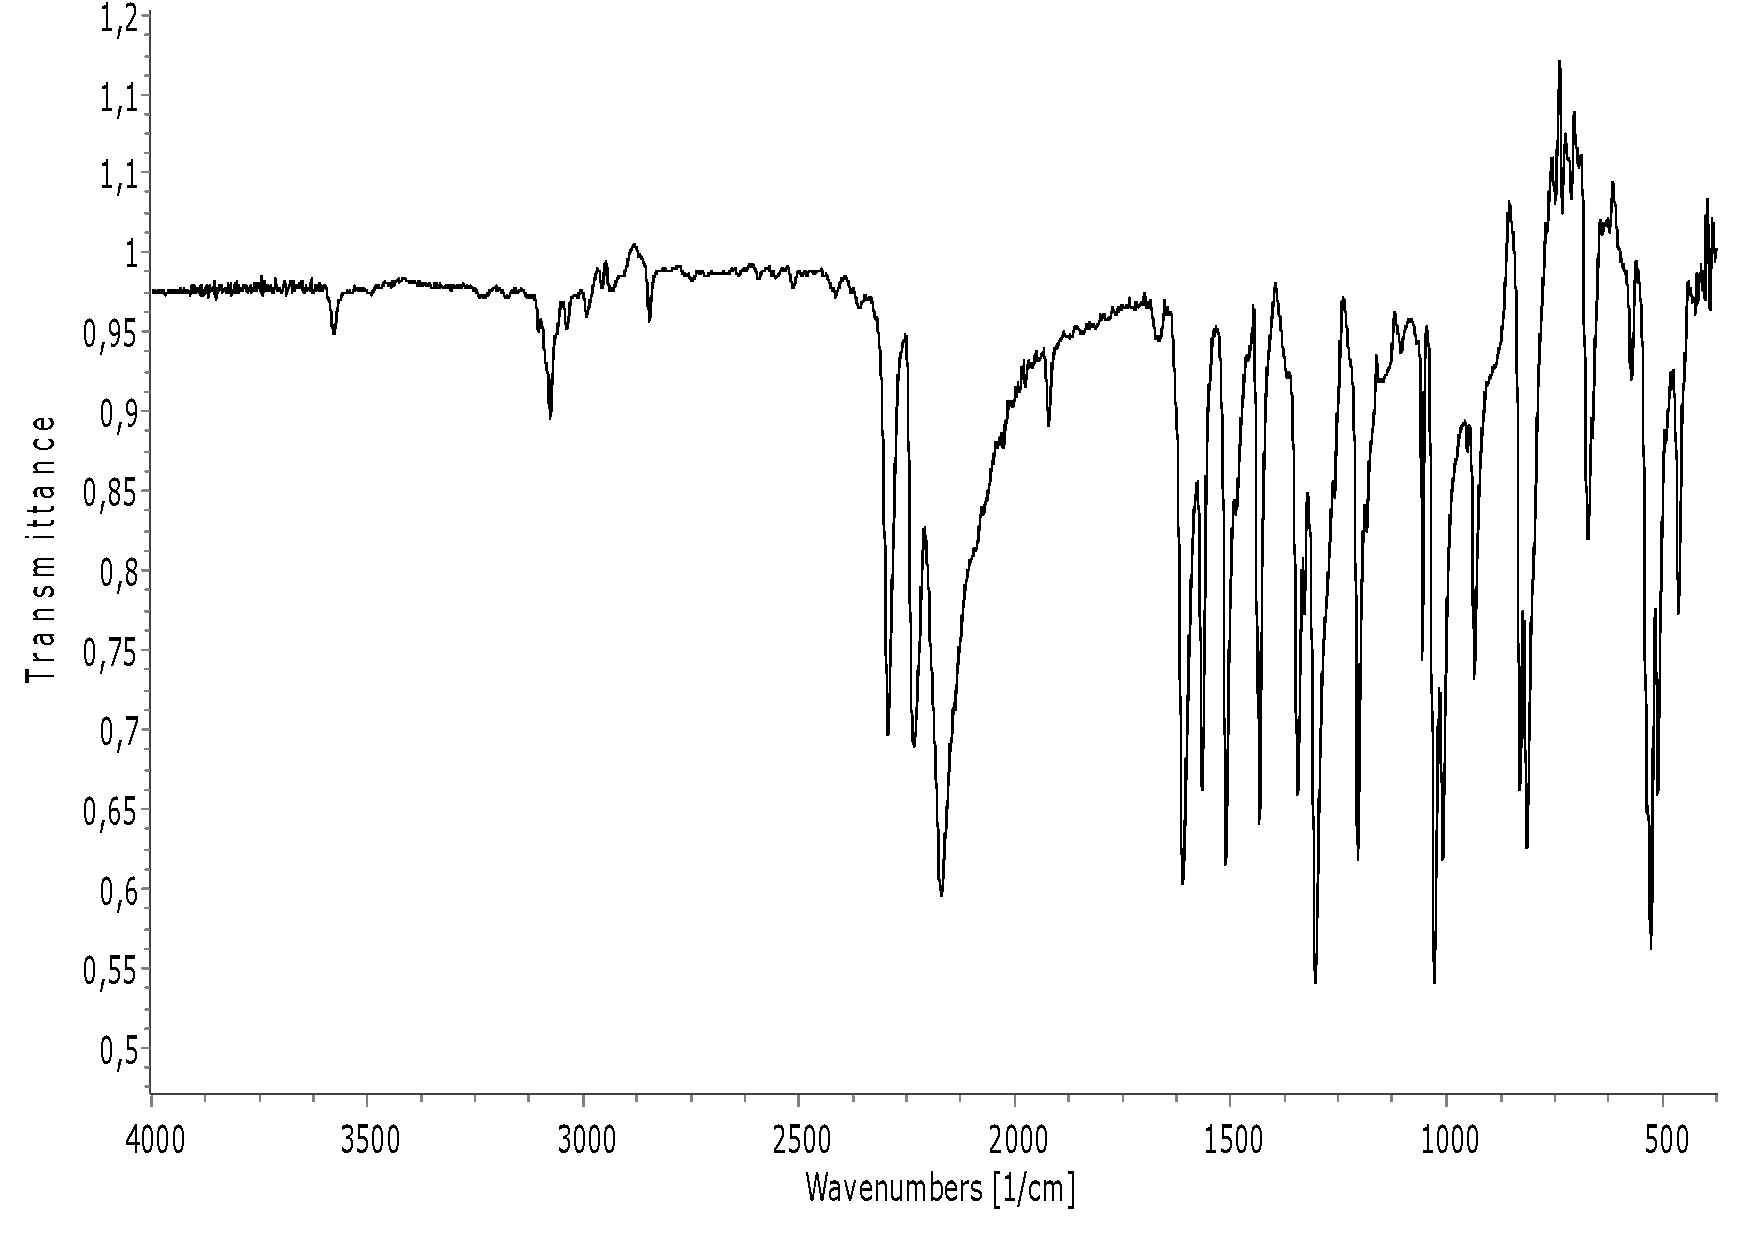
\includegraphics[width=1\textwidth]{figures/ZnD4MOP-IR.pdf}
\caption{IR-Spectrum of \ce{[Zn(dca)_2(4-MeOpy)_2]_n}}
\end{figure}

\subsection{Structural characterization}


The selected bond parameters of \ce{[Zn(dca)_2(4-MeOpy)_2]_n} are summarized in table \ref{batab:ZnD4MOP}. Its crystal structure is displayed in fig. \ref{fig:ZnD4MOP_pv} (perspective view) and fig. \ref{fig:ZnD4MOP_packv} (packing view).  Zn(1) is situated on an inversion center and connected to six ligands: four of them are dicyanamide anions which act in bis-$\mu$(1,5)-bridging mode, forming a polymeric chain along the axis of the triclinic cell. The others are 4-MOP molecules in trans configuration. The \ce{ZnN_6} polyhedron forms an almost regular octahedron, with Zn-N bond distances varying from 2.1288(15) to 2.1733(19) \AA, and a maximum deviation of 0.89$^\circ$ of the N-Zn-N bond angles from 90 or 180$^\circ$. The dicyanamide bridges have the following bond parameters: Zn-N-C: 162.01(18) and 159.00(19)$^\circ$; N-C-N: 174.9(2) and 175.6(2)$^\circ$; C-N-C: 118.38(17)$^\circ$; C-N(nitril) 1.154(3) and 1.158(3) \AA; C-N(amide): 1.310(3) and 1.309(3) \AA. The intra-chain Zn\ce{***}Zn distance of 7.3706(4) \AA \ \ is longer than the shortest inter-chain metal\ce{***}metal separation of 7.0620(4) \AA. 

\renewcommand{\arraystretch}{1.5}

\begin{table}[htpb!]
\centering
\captionabove{Selected bond lengths (\AA) and angles ($^\circ$) for \ce{[Zn(dca)_2(4-MeOpy)_2]_n}; Symmetry codes: (a) 2-x, 2-y, -z; (b) 2-x, 1-y, -z; (c) x, 1+y, z; (d) x, -1+y, z; (e) 2-x, 3-y; -z; (f) 2-x, -y, -z.}
\begin{tabular}{|l|l|l|l|}
\hline
Zn(1)-N(1a) & 2.1288(15) & Zn(1)-N(4b) & 2.1733(19)\\
\hline
Zn(1)-N(2a) & 2.1710(19)& N(3)-C(7) & 1.310(3)\\
\hline
N(2)-C(7) & 1.154(3) & N(3)-C(8) & 1.309(3)\\
\hline
N(4)-C(8) & 1.158(3) &  & \\
\hline
\hline
N(1)-Zn(1)-N(2a) & 90.59(7) & N(1a)-Zn(1)-N(4b) & 90.28(7)\\
\hline
N(4c)-Zn(1)-N(2a) & 90.89(6) & N(2)-Zn(1)-N(2a) & 180.0\\
\hline
Zn(1)-N(2)-C(7) & 162.01(18) & N(2)-C(7)-N(3) & 174.9(2)\\
\hline
Zn(1b)-N(4)-C(8)& 159.00(19) &N(4)-C(8)-N(3) & 175.6(2)\\
\hline
C(7)-N(3)-C(8)& 118.38(17) & &\\
\hline
\end{tabular}
\label{batab:ZnD4MOP}
\end{table}


\begin{figure}[!htpb]
\centering
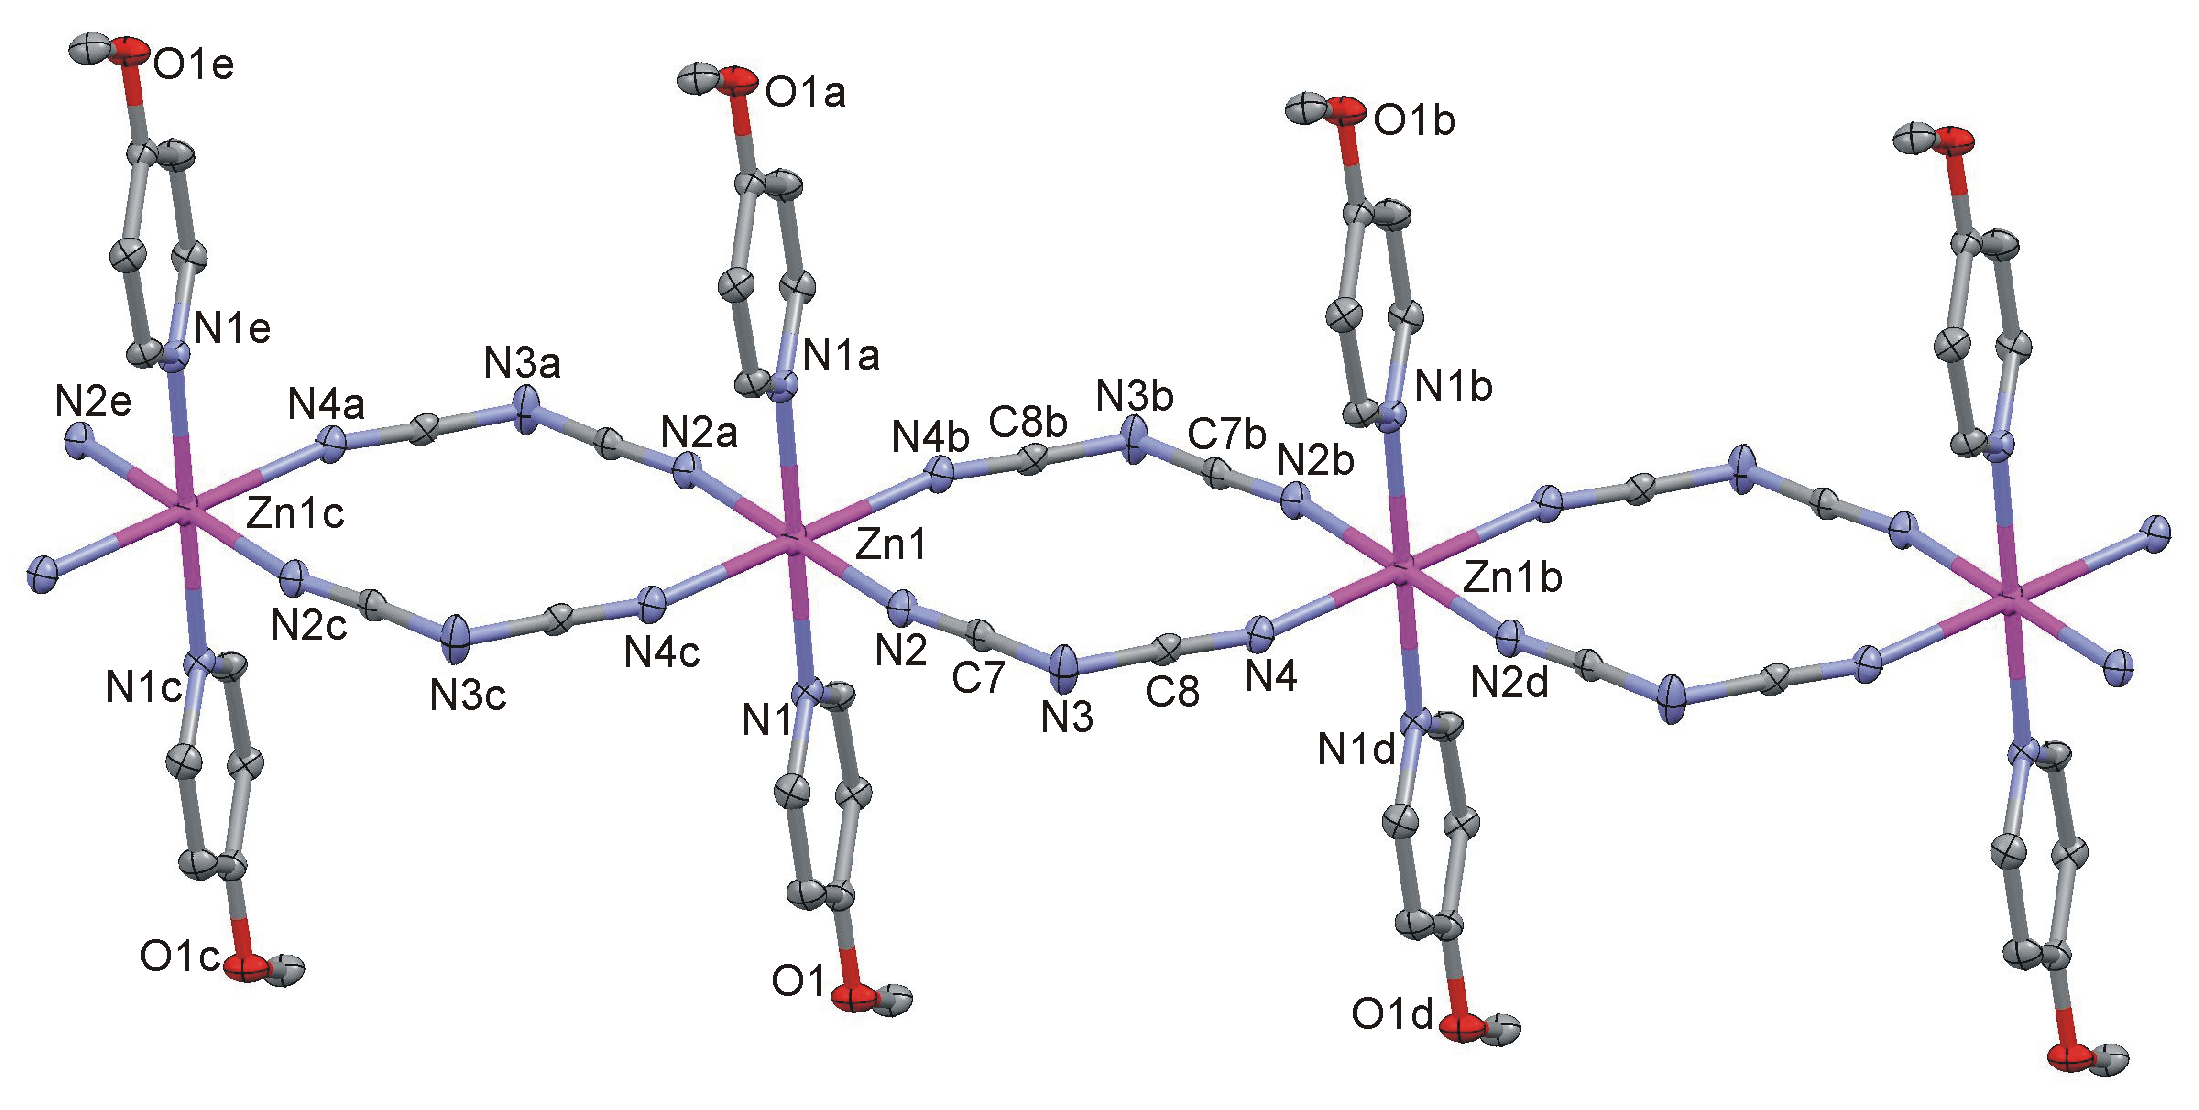
\includegraphics[width=1\textwidth]{figures/ZnD_4MOP_FIGm11.png}
\caption[Perspective view of \ce{[Zn(dca)_2(4-MeOpy)_2]_n}]{Perspective view of a section of the polymeric chain of \ce{[Zn(dca)_2(4-MeOpy)_2]_n} together with the atom numbering scheme. Symmetry codes: (a) 2-x,2-y,-z; (b) 2-x,1-y,-z; (c) x,1+y,z; (d) x,-1+y,z; (e) 2-x,3-y,-z; (f) 2-x,-y,-z.}
\label{fig:ZnD4MOP_pv}
\vspace{\floatsep}
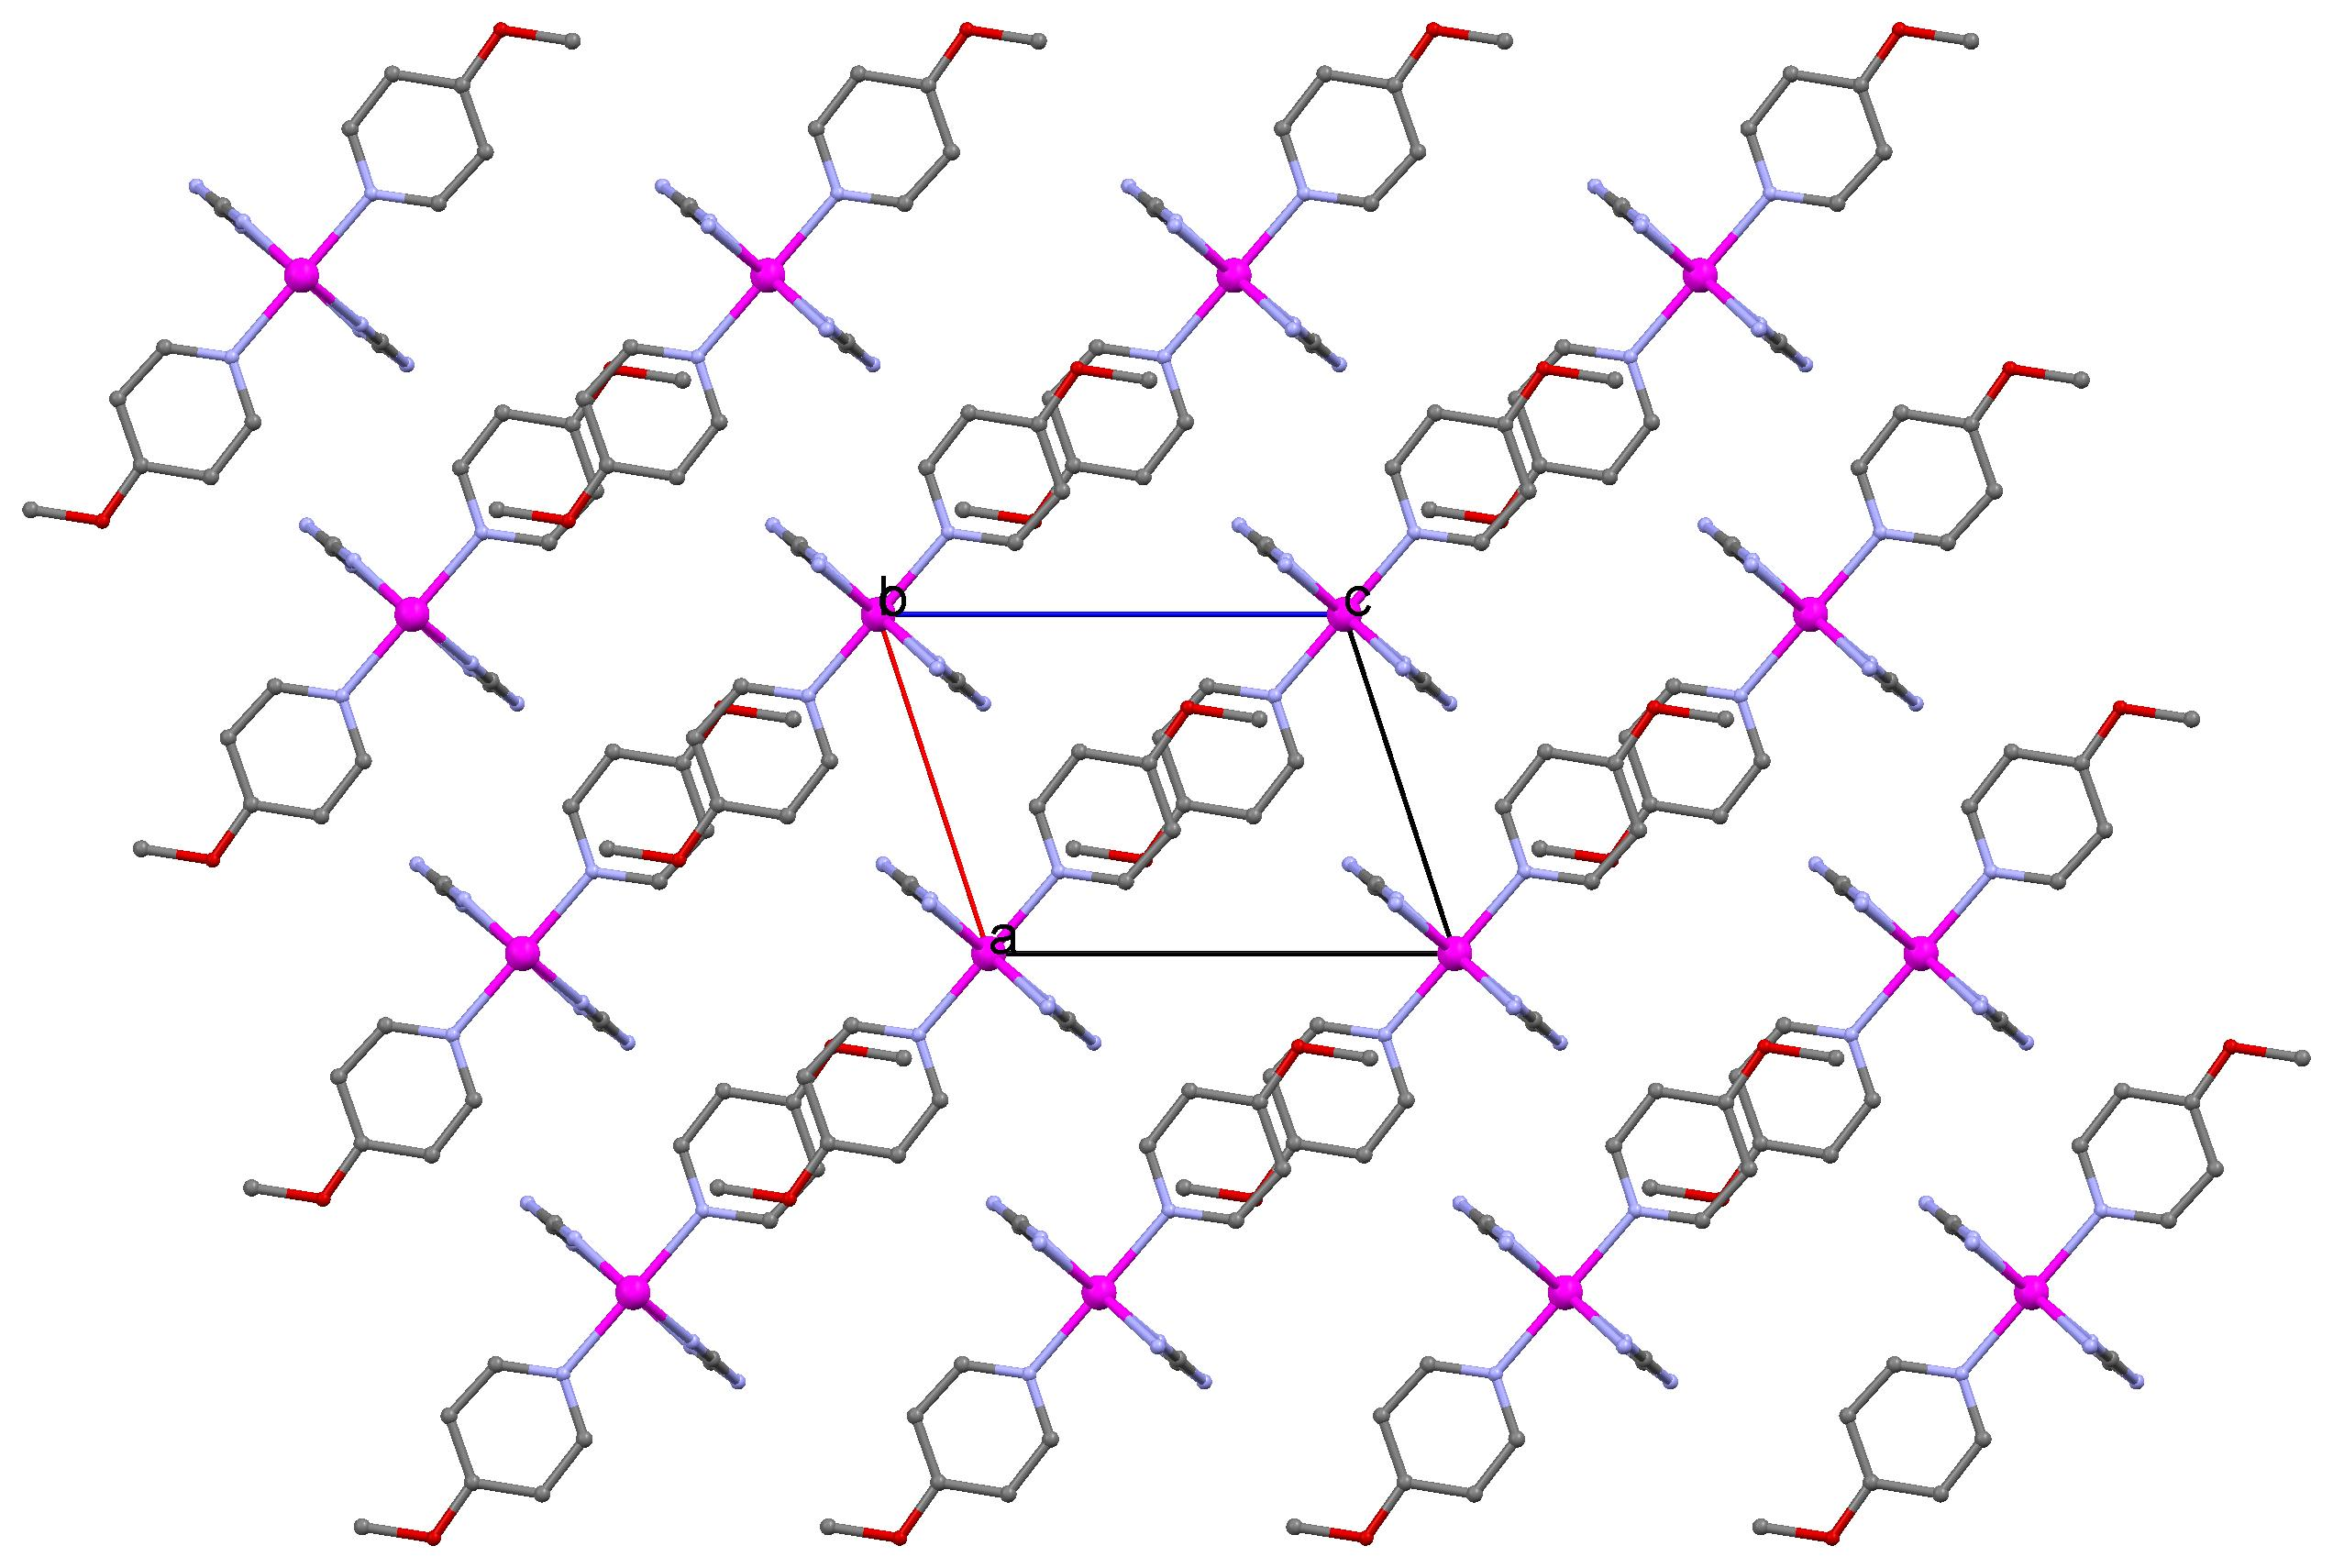
\includegraphics[width=1\textwidth]{figures/znd_4mop_CB.png}
\caption{Packing plot  of \ce{[Zn(dca)_2(4-MeOpy)_2]_n}.}
\label{fig:ZnD4MOP_packv}
\end{figure}



\begin{table}
\centering
\captionabove{Crystallographic data and processing parameter of \ce{[Zn(dca)_2(4-MeOpy)_2]_n}.}
\begin{tabular}{ | l |  l | }
\hline
Empirical formula & \ce{C_{16}H_{14}N_{8}O_{2}Zn}\\
\hline
Formula mass & 415.74\\
\hline
System & triclinic\\
\hline
Space group & P-1\\
\hline
a ({\AA}) & 7.0620(4)\\
\hline
b ({\AA}) & 7.3706(4)\\
\hline
c ({\AA}) & 9.8134(5)\\
\hline
$\alpha$ ($^\circ$) & 69.847(2)\\
\hline
$\beta$ ($^\circ$) & 71.759(3)\\
\hline
$\gamma$ ($^\circ$) & 86.183(3)\\
\hline
V (\AA$^{3}) $  & 454.94(4)\\
\hline
Z & 1\\
\hline
T (K) & 100(2)\\
\hline
$\mu$ (mm$^{-1}$) & 1.379\\
\hline
 D$_{calc}$ (Mg/m$^{3}$) & 1.518\\
\hline
Crystal size (mm) & 0.26 x 0.21 x 0.12\\
\hline
$\theta$ max ($^\circ$) & 28.00\\
\hline
Data collected & 2188\\
\hline
Unique refl./ R$_{int}$ & 2188 / ----\\
\hline
Parameters & 126\\
\hline
Goodness-of-Fit on F$^{2}$ & 1.148\\
\hline
R1 / wR2 (all data) & 0.0282 /0.0798\\
\hline
Residual extrema (e/\AA$^{3}$) & 0.40 /-0.40\\
\hline
\end{tabular}

\label{ptab:ZnD4MOP}

\end{table}


 

